\documentclass{article}
\usepackage[utf8]{inputenc}
\usepackage{subfig}
\usepackage{amsmath}

\usepackage{graphicx}
\usepackage[legalpaper, landscape, margin=0.5cm]{geometry}

\thispagestyle{empty}
% \renewcommand{\thesubfigure}{\roman{subfigure}}
\begin{document}

\begin{figure}[h]
        \centering
        \subfloat[vertical caustics]{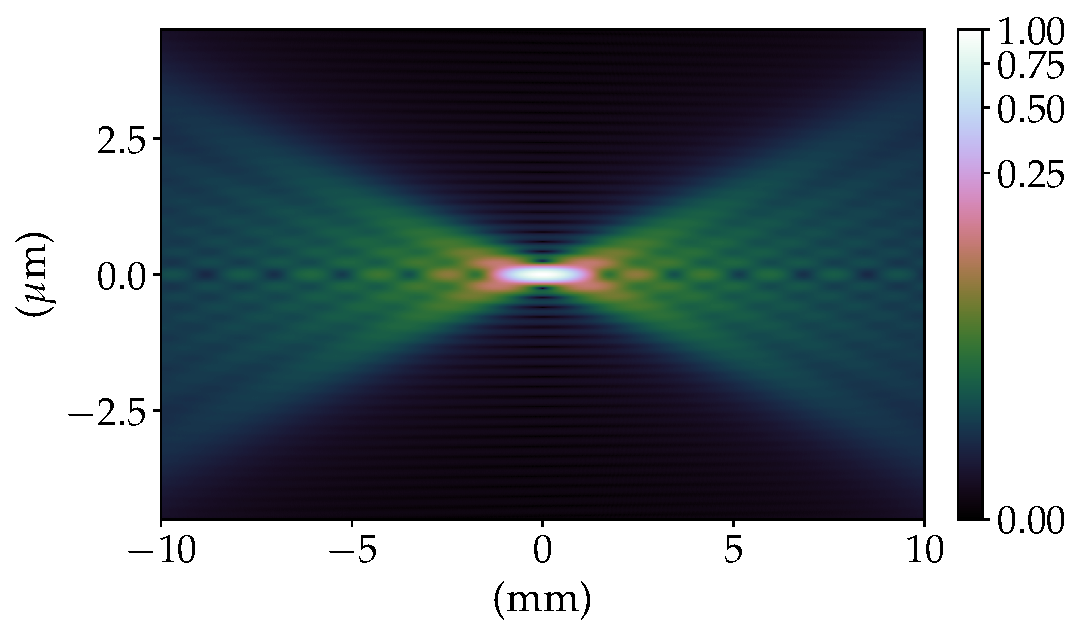
\includegraphics[height=3.4cm]{figures/ch05/CDn_vs_CDnStack/Be_ideal_8p0keV_d0p0mm_n10_intensity_cstc_Y_cstc_2D.pdf}}\hspace{0.1cm}
        \subfloat[PSF phase (rad)]{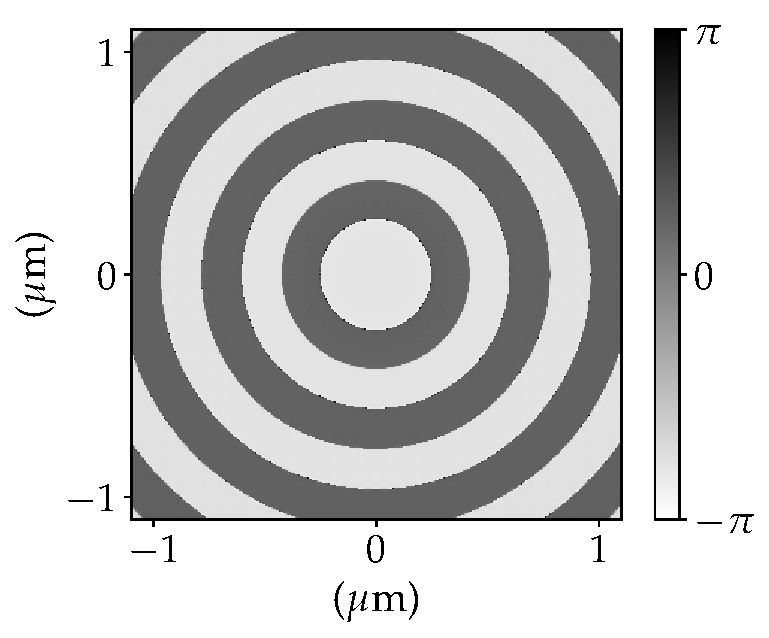
\includegraphics[height=3.5cm]{figures/ch05/CDn_vs_CDnStack/Be_ideal_8p0keV_d0p0mm_n10_phase_phase_2D.pdf}}\hspace{0.1cm}
        \subfloat[PSF intensity]{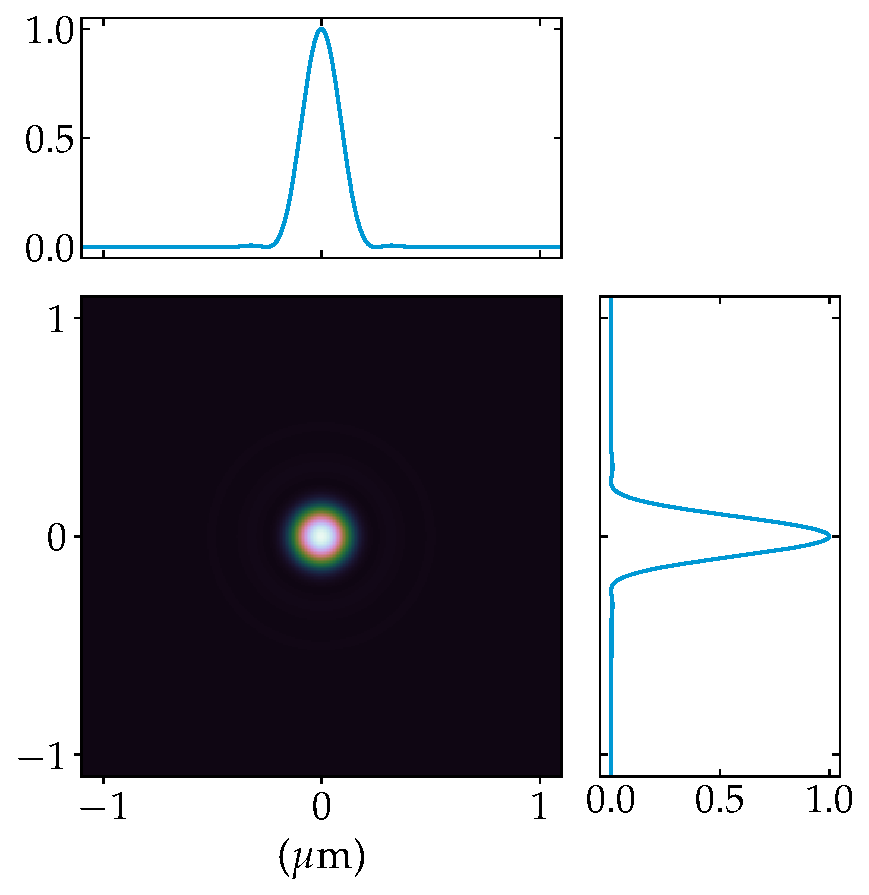
\includegraphics[height=5cm]{figures/ch05/CDn_vs_CDnStack/Be_ideal_8p0keV_d0p0mm_n10_intensity_intensity_2D.pdf}}\hspace{0.1cm}
        \subfloat[source image]{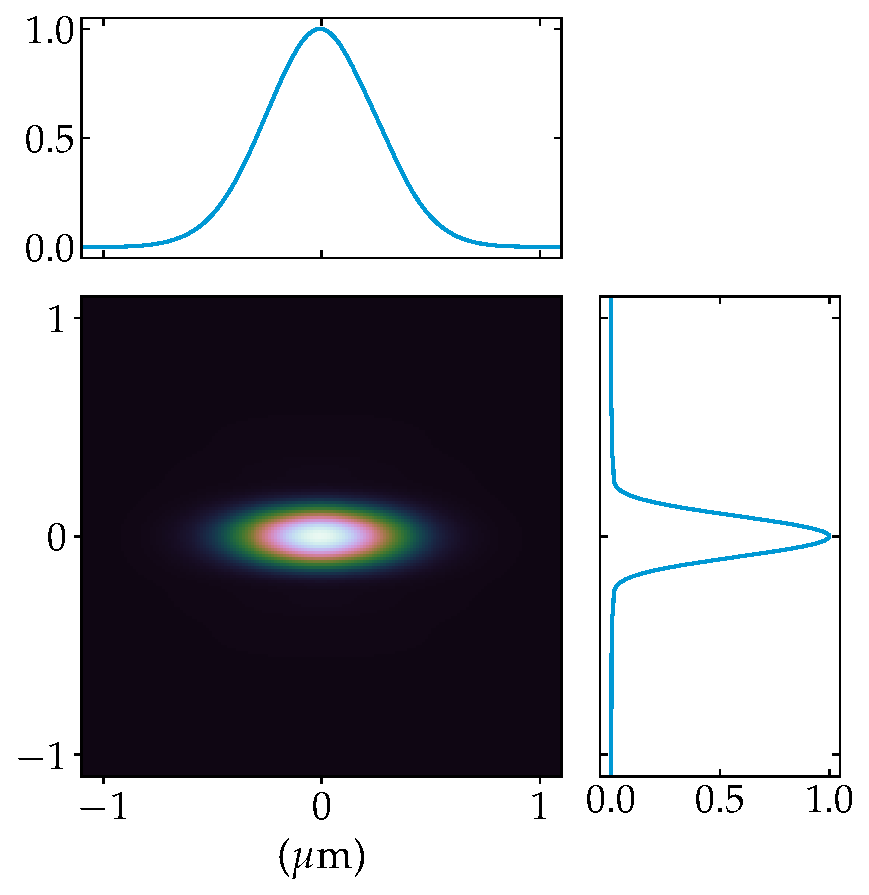
\includegraphics[height=5cm]{figures/ch05/CDn_vs_CDnStack/Be_ideal_8keV_d0p0mm_10k_ME_intensity_intensity_2D.pdf}}
\end{figure}
\end{document}